\documentclass[a4paper, 12pt]{article}
\usepackage[utf8]{inputenc}
\usepackage[russian,english]{babel}
\usepackage[T2A]{fontenc}
\usepackage[left=10mm, top=20mm, right=10mm, bottom=15mm, footskip=13mm]{geometry}
\usepackage{indentfirst}
\usepackage{amsmath,amssymb}
\usepackage{graphicx}
\usepackage[italicdiff]{physics}
\usepackage{float}
\usepackage{array}
\usepackage{physics}
\graphicspath{ {shema/} {graphic/} }
\usepackage{caption}
\captionsetup[figure]{name=Рисунок}
  
\title{Отчет по лабораторной работе 1.3.2

Определение модуля кручения}

\author{Максим Осипов, Б03-504}
\date{01.10.2025}

\begin{document}
\maketitle
\newpage

\section{Аннотация}
 Цель работы: измерение углов закручивания в зависимости от приложенного момента сил, расчет
 модулей кручения и сдвига при статическом закручивании стержня, определение тех же модулей
 для проволоки по измерениям периодов крутильных колебаний подвешенного на ней маятника (ди
намическим методом).\\
\indent
 В работе используются: в первой части: исследуемый стержень, отсчетная труба со шкалой,
 рулетка, микрометр, набор грузов; во второй части: проволока из исследуемого материала, грузы,
 секундомер, микрометр, рулетка, линейка.

\section{Теоретическая справка}

1. Чистое кручение цилиндрического стержня

При закручивании цилиндрических стержней круглого сечения в областях, удаленных от мест приложения закручивающих моментов, возникает напряженное состояние, называемое чистым кручением. В этом состоянии каждое поперечное сечение поворачивается как жесткое целое, при этом:
- Частицы материала не смещаются с радиальных линий
- Все радиальные линии поворачиваются на одинаковый угол
- Касательные напряжения увеличиваются пропорционально расстоянию от оси вращения

\begin{figure}[h]
\centering
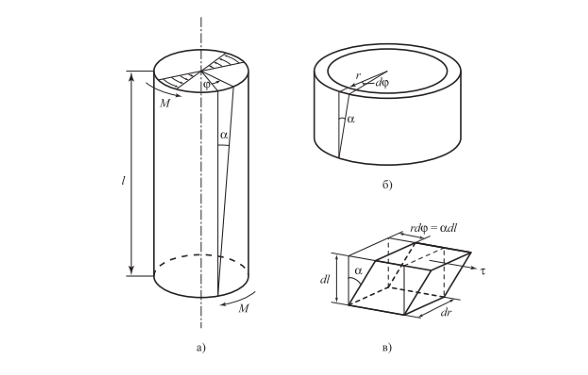
\includegraphics[width=0.8\linewidth]{рис 1.png}
\caption{Закручивание цилиндра}
\label{fig:voltage_current}
\end{figure}


2. Основные соотношения при кручении

Рассмотрим цилиндр длиной \( l \), у которого сечения, находящиеся на расстоянии \( l \), повернуты на угол \( \varphi \). Для элементарного колечка радиуса \( r \) с толщиной \( dr \) и высотой \( dl \) выполняется соотношение:
\[
\alpha dl = rd\varphi.\tag{1}
\]

где \( \alpha \) - угол сдвига, характеризующий наклон образующей цилиндрической поверхности.

Касательное напряжение \( \tau \) связано с углом сдвига \( \alpha \) через модуль сдвига \( G \):
\[
\tau = G\alpha.\tag{2}
\]


Из (1) и (2) следует, что касательное напряжение пропорционально расстоянию от оси:
\[
\tau = Gr\frac{d\varphi}{dl}.\tag{3}
\]


3. Момент сил при кручении

Элементарный момент сил, создаваемый касательными напряжениями на кольце радиуса \( r \):
\[
dM = 2\pi rdr \cdot \tau \cdot r.\tag{4}
\]


Суммарный момент сил по всему поперечному сечению:
\[
M = 2\pi G \frac{d\varphi}{dl} \int_{0}^{R} r^3 dr = \pi G \frac{d\varphi}{dl} \frac{R^4}{2}.\tag{5}
\]


4. Модуль кручения

Из (5) получаем линейную зависимость между моментом сил \( M \) и углом закручивания \( \varphi \):
\[
M = \frac{\pi R^4 G}{2l} \varphi = f\varphi.\tag{6}
\]


где введен модуль кручения \( f \), связанный с модулем сдвига \( G \):
\[
f = \frac{\pi R^4 G}{2l}.\tag{7}
\]


\subsection{Крутильные колебания}

Для системы, совершающей крутильные колебания на проволоке, уравнение движения имеет вид:
\[
I \frac{d^2 \varphi}{dt^2} = -M.\tag{8}
\]

где \( I \) - момент инерции системы относительно оси вращения.

При малых углах закручивания, используя (6), получаем:
\[
\frac{d^2 \varphi}{dt^2} + \omega^2 \varphi = 0.\tag{10}
\]

где
\[
\omega^2 = \frac{f}{I}.
\]


Решение уравнения (10) описывает гармонические колебания:
\[
\varphi = \varphi_0 \sin(\omega t + \theta).\tag{11}
\]


Период крутильных колебаний:
\[
T = \frac{2\pi}{\omega} = 2\pi \sqrt{\frac{I}{f}}.\tag{12}
\]


5. Роль теоретических положений в эксперименте

- Формула (6) является рабочей для статического метода: измеряя угол закручивания \( \varphi \) при известном моменте \( M \), можно определить модуль кручения \( f \), а затем по (7) вычислить модуль сдвига \( G \)

- Формула (12) является рабочей для динамического метода: измеряя период колебаний \( T \) системы с известным моментом инерции \( I \), можно определить модуль кручения \( f \), а затем модуль сдвига \( G \)

- Условие малых углов \( \alpha \) обеспечивает применимость линейной зависимости (2) и выполнение закона Гука для сдвига

- Условие незатухающих колебаний (уменьшение амплитуды менее чем в 2 раза за 10 периодов) позволяет использовать формулу (12) для точного определения периода

- Независимость периода от амплитуды подтверждает применимость теории малых колебаний

\section{Установка}


\begin{figure}[h]
\centering
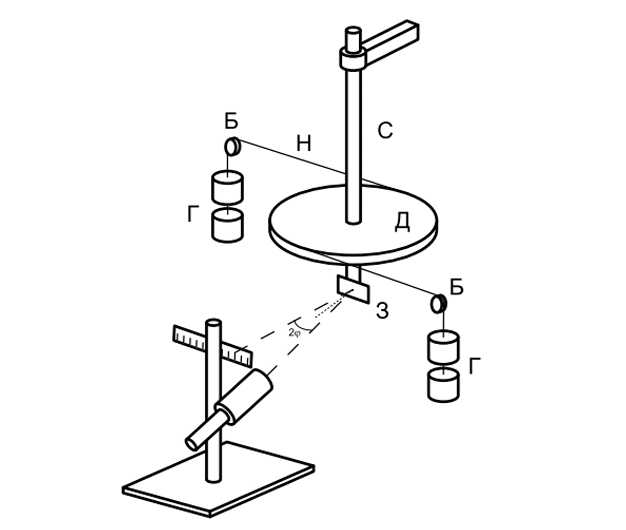
\includegraphics[width=0.4\linewidth]{схема установки1.png}
\caption{Схема установки для статического закручивания }
\label{fig:voltage_current}
\end{figure}

\begin{figure}[h]
\centering
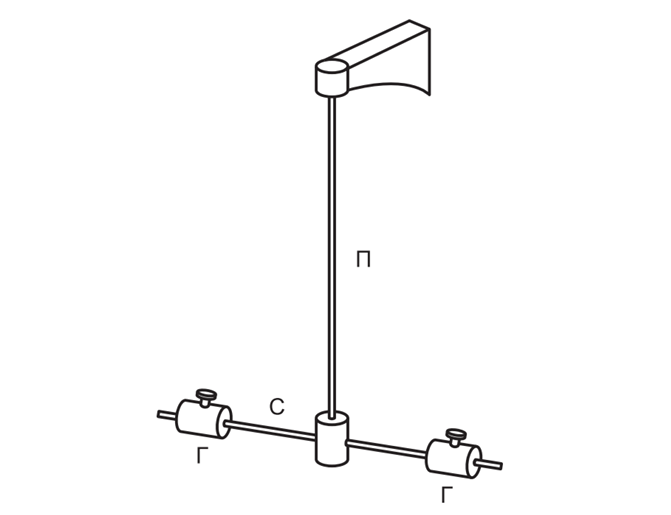
\includegraphics[width=0.4\linewidth]{схема установки2.png}
\caption{Схема установки для крутильных колебаний }
\label{fig:voltage_current}
\end{figure}



\end{document}
